\section{Dataset}
\label{sec:data}

As mentioned in the introduction, the dataset of the COVID-19 outbreak in Italy is used to test the mathematical model. The Italian spreading of the virus is measured through different quantities, reported in Figure~\ref{fig:data_italy}. The numbers refer to people that has been tested for the virus. In the following, a person with a positive outcome of the test, meaning infected by the virus, is also called as a \emph{positive case}.  \\

Tests have been performed on population showing heavy symptoms and hospitalised, but also on the medical staff. In some cases, also close connections to those individuals are also tested. This strategy has been quite restrictive and constant, due to a lack of available test kits. As the Figure~\ref{fig:data_italy} shows, a positive person dies or recover. The total cases per day are given by the sum of current positively tested individuals, deaths and recovered.\\

However, the dataset used to test the model refers are collected only in Lombardy. This region has been the first region where the virus spread and the most affected one. Moreover most of the cases, especially at the beginning, were registered in this region, being the largest contrbution in the overall Italian dataset. The data of the total cases versus time in the Lombardy area are shown in Figure~\ref{fig:data_lombardy}. The shown data are extracted from the web-site of \emph{Il Sole 24 Ore} \cite{Lab24}, the main economical italian newspaper, that has been one of the first sources of data of the outbreak in Italy divided by regions. \\

\begin{figure}[!ht]\centering
\subfloat[\label{fig:data_italy}]{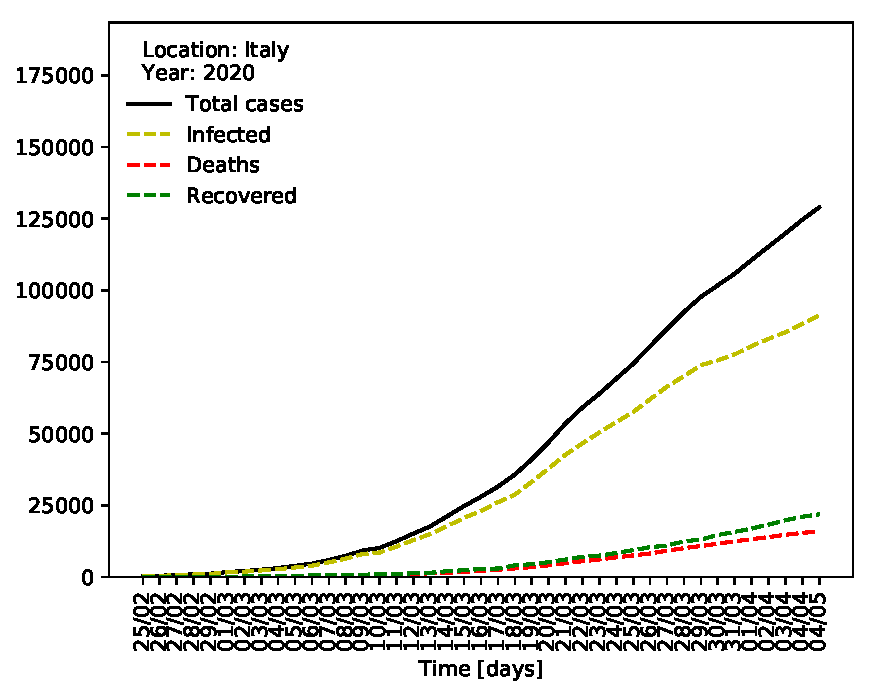
\includegraphics[width=0.4\textwidth]{imgs/Dataset/Data_Italy.pdf}}
\subfloat[\label{fig:data_lombardy}]{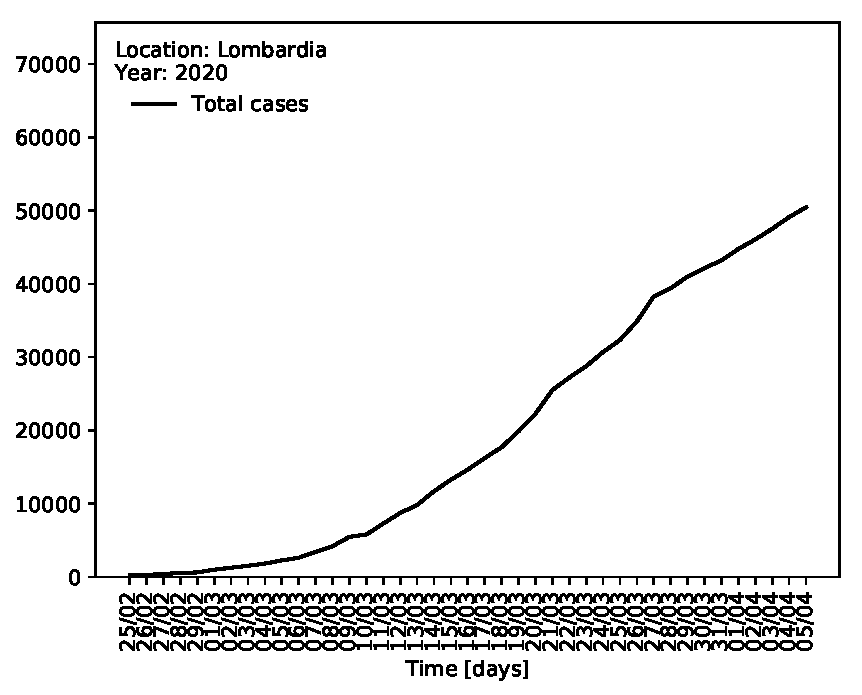
\includegraphics[width=0.4\textwidth]{imgs/Dataset/Data_Lombardia.pdf}}

\caption{Dataset collected in Italy (a) and Lombardy (b).}.
\end{figure}

The reason because only Lombardy has been chosen to test the model are several. As mentioned above, it is not restrictive since it is by far the most affected region in Italy. Moreover, sanitary procedures are managed at regional level, therefore there is a more consistent choice of strategy to contain the outbreak. Finally, it is smaller than the whole country, high-populated, very dynamic and connected area, where small-world approximation is a better assumption.